\documentclass[]{scrartcl}

\usepackage{minted}
\usepackage{mdframed}  
\usepackage{xcolor}
\usepackage{tikz}
\usepackage{tikz-3dplot}
\usetikzlibrary{matrix,decorations.pathreplacing, calc, positioning,fit}

\surroundwithmdframed[linewidth=0pt, backgroundcolor=black!10]{minted} 

\newcommand{\draftNote}[1]
{
	\begin{mdframed}[linewidth=0pt, backgroundcolor=red!10]
		#1
	\end{mdframed}
}


\newcommand{\draftNoteInline}[1]
{
	\textcolor{red}{(#1)}
}

\newcommand{\cppInline}[1]
{
	\mintinline{cpp}{#1}
}


\newcommand{\plotSwizzleTwoRegisters}[8]
{
	\matrix [matrix of math nodes,
	left delimiter={[},
	right delimiter={]},
	](A) at (0,0){ 
		|[fill=red!20]|\mathbf{a_{0}}\\
		|[fill=red!40]|\mathbf{a_{1}}\\  
		|[fill=red!60]|\mathbf{a_{2}}\\
		|[fill=red!80]|\mathbf{a_{3}}\\
		\textbf{---}\\
		|[fill=blue!15]|\mathbf{a_{4}}\\
		|[fill=blue!30]|\mathbf{a_{5}}\\
		|[fill=blue!55]|\mathbf{a_{6}}\\
		|[fill=blue!70]|\mathbf{a_{7}}\\
	};
	
	\matrix [matrix of math nodes,
	left delimiter={[},
	right delimiter={]},
	](B) at (5,0){ 
		|[fill=#1]|\mathbf{b_{0}}\\
		|[fill=#2]|\mathbf{b_{1}}\\  
		|[fill=#3]|\mathbf{b_{2}}\\
		|[fill=#4]|\mathbf{b_{3}}\\
		|[fill=white]|\textbf{---}\\
		|[fill=#5]|\mathbf{b_{4}}\\
		|[fill=#6]|\mathbf{b_{5}}\\
		|[fill=#7]|\mathbf{b_{6}}\\
		|[fill=#8]|\mathbf{b_{7}}\\
	};
}



\newcommand{\plotSwizzleThreeRegisters}[8]
{
	\matrix [matrix of math nodes,
	left delimiter={[},
	right delimiter={]},
	column 1/.style = {nodes={fill=red!50}},
	](A) at (0,0){ 
		\mathbf{a_{0}}\\
		\mathbf{a_{1}}\\  
		\mathbf{a_{2}}\\
		\mathbf{a_{3}}\\
		|[fill=white]|\textbf{---}\\
		\mathbf{a_{4}}\\
		\mathbf{a_{5}}\\
		\mathbf{a_{6}}\\
		\mathbf{a_{7}}\\
	};

	\matrix [matrix of math nodes,
	left delimiter={[},
	right delimiter={]},
	column 1/.style = {nodes={fill=blue!50}},
	](B) at (10,0){ 
		\mathbf{b_{0}}\\
		\mathbf{b_{1}}\\  
		\mathbf{b_{2}}\\
		\mathbf{b_{3}}\\
		|[fill=white]|\textbf{---}\\
		\mathbf{b_{4}}\\
		\mathbf{b_{5}}\\
		\mathbf{b_{6}}\\
		\mathbf{b_{7}}\\
	};

	\matrix [matrix of math nodes,left delimiter={[},right delimiter={]}](C) at (5,0){ 
		|[fill=#1!50]|\mathbf{c_{0}}\\
		|[fill=#2!50]|\mathbf{c_{1}}\\  
		|[fill=#3!50]|\mathbf{c_{2}}\\
		|[fill=#4!50]|\mathbf{c_{3}}\\
		|[fill=white]|\textbf{---}\\
		|[fill=#5!50]|\mathbf{c_{4}}\\
		|[fill=#6!50]|\mathbf{c_{5}}\\
		|[fill=#7!50]|\mathbf{c_{6}}\\
		|[fill=#8!50]|\mathbf{c_{7}}\\
	};
}


%opening
\title{Documentation of swizzle and transpose functions for x86 vector registers}
\author{vhirtham}

\begin{document}		
\maketitle
\section*{About this document}
The purpose of this document is to give a short overview over the available swizzle instructions for x86 register types and the \mintinline{cpp}{Transpose} functions for matrices based on x86 vector registers.


\section{Swizzle operations}
\draftNote{
\begin{itemize}
\item Mention why template parameters -> compile time constants
\end{itemize}
}

\subsection{AlignRight}

\subsection{Blending}

A blend operation conditionally copies the data elements from either the first or second input registers to the same position inside a result register. 
The underlying x86 intrinsic function are \cppInline{_mm_blend_ps}, \cppInline{_mm_blend_pd}, \cppInline{_mm256_blend_ps} and \cppInline{_mm256_blend_pd}.
These functions need an integer as parameter that controls the value selection.
Several functions that calculate the control integer value based on chosen template parameters are implemented.
So it is not necessary to determine the correct integer value yourself.

On current x86 CPU architectures, blending is the most efficient swizzle operation, since multiple blends can be performed during a single CPU cycle.

\subsubsection{Blend}

The \cppInline{Blend} function has as many template parameters as data elements.
Each value van either be 0 or 1.
If a template parameter is set to 0, the corresponding data element receives its value from the first source register.
If it is 1, the value is taken from the second input register.

\subsubsection*{Example:}
\begin{minted}{cpp}
__m256 c = Blend<0, 1, 1, 0, 1, 0, 0, 0>(a, b)
\end{minted}

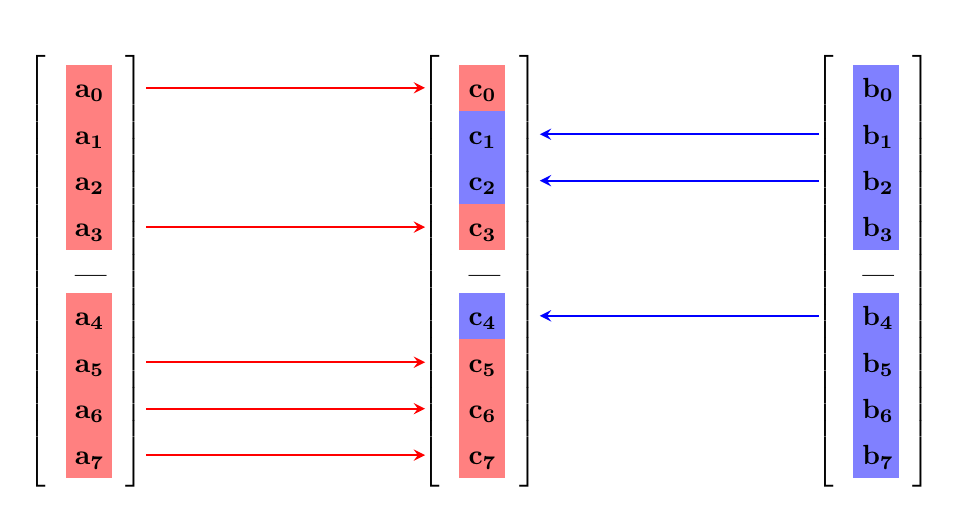
\begin{tikzpicture}[>=stealth,thick,baseline, every node/.style={text height=2ex,text width=1em}]
\plotSwizzleThreeRegisters{red}{blue}{blue}{red}{blue}{red}{red}{red}

\draw[->,color=red ]([xshift= 12pt]A-1-1.east)-- ([xshift=-12pt]C-1-1.west);
\draw[->,color=blue]([xshift=-12pt]B-2-1.west)-- ([xshift= 12pt]C-2-1.east);
\draw[->,color=blue]([xshift=-12pt]B-3-1.west)-- ([xshift= 12pt]C-3-1.east);
\draw[->,color=red ]([xshift= 12pt]A-4-1.east)-- ([xshift=-12pt]C-4-1.west);
\draw[->,color=blue]([xshift=-12pt]B-6-1.west)-- ([xshift= 12pt]C-6-1.east);
\draw[->,color=red ]([xshift= 12pt]A-7-1.east)-- ([xshift=-12pt]C-7-1.west);
\draw[->,color=red ]([xshift= 12pt]A-8-1.east)-- ([xshift=-12pt]C-8-1.west);
\draw[->,color=red ]([xshift= 12pt]A-9-1.east)-- ([xshift=-12pt]C-9-1.west);
\end{tikzpicture}


\subsubsection{BlendIndex}

The \cppInline{BlendIndex} function has only a single template parameter independent of the used register types' size.
It specifies the index of a single data element that is taken from the second source register. 
All other values are taken from the first one.

\subsubsection*{Example:}
\begin{minted}{cpp}
__m256 c = BlendIndex<5>(a, b)
\end{minted}


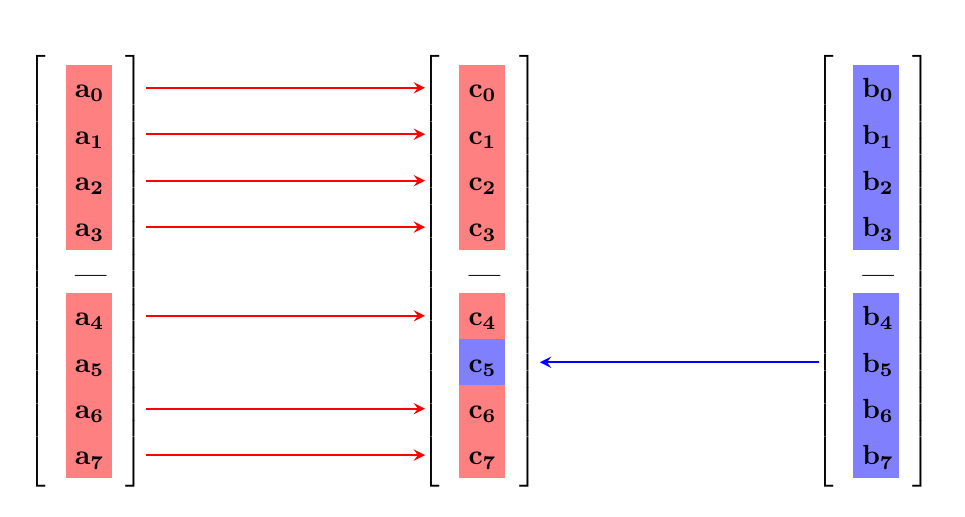
\begin{tikzpicture}[>=stealth,thick,baseline, every node/.style={text height=2ex,text width=1em}]
\plotSwizzleThreeRegisters{red}{red}{red}{red}{red}{blue}{red}{red}

\draw[->,color=red ]([xshift= 12pt]A-1-1.east)-- ([xshift=-12pt]C-1-1.west);
\draw[->,color=red ]([xshift= 12pt]A-2-1.east)-- ([xshift=-12pt]C-2-1.west);
\draw[->,color=red ]([xshift= 12pt]A-3-1.east)-- ([xshift=-12pt]C-3-1.west);
\draw[->,color=red ]([xshift= 12pt]A-4-1.east)-- ([xshift=-12pt]C-4-1.west);
\draw[->,color=red ]([xshift= 12pt]A-6-1.east)-- ([xshift=-12pt]C-6-1.west);
\draw[->,color=blue]([xshift=-12pt]B-7-1.west)-- ([xshift= 12pt]C-7-1.east);
\draw[->,color=red ]([xshift= 12pt]A-8-1.east)-- ([xshift=-12pt]C-8-1.west);
\draw[->,color=red ]([xshift= 12pt]A-9-1.east)-- ([xshift=-12pt]C-9-1.west);
\end{tikzpicture}


\subsubsection{BlendAboveIndex}

The \cppInline{BlendIndex} function has only a single template parameter independent of the used register types' size.
Data elements with a higher index than the specified value are taken from the second source register. 
All other values are taken from the first one.

\subsubsection*{Example:}
\begin{minted}{cpp}
__m256 c = BlendAboveIndex<5>(a, b)
\end{minted}

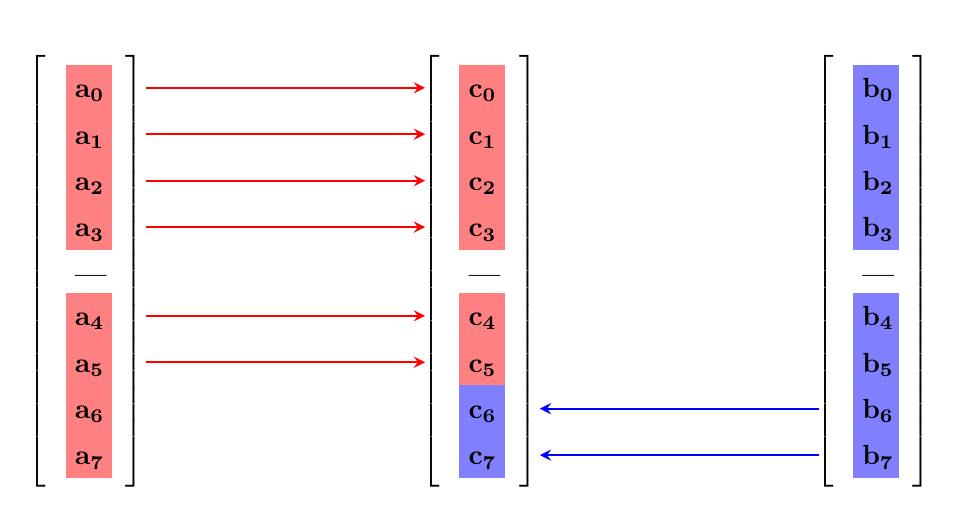
\begin{tikzpicture}[>=stealth,thick,baseline, every node/.style={text height=2ex,text width=1em}]
\plotSwizzleThreeRegisters{red}{red}{red}{red}{red}{red}{blue}{blue}

\draw[->,color=red ]([xshift= 12pt]A-1-1.east)-- ([xshift=-12pt]C-1-1.west);
\draw[->,color=red ]([xshift= 12pt]A-2-1.east)-- ([xshift=-12pt]C-2-1.west);
\draw[->,color=red ]([xshift= 12pt]A-3-1.east)-- ([xshift=-12pt]C-3-1.west);
\draw[->,color=red ]([xshift= 12pt]A-4-1.east)-- ([xshift=-12pt]C-4-1.west);
\draw[->,color=red ]([xshift= 12pt]A-6-1.east)-- ([xshift=-12pt]C-6-1.west);
\draw[->,color=red ]([xshift= 12pt]A-7-1.east)-- ([xshift=-12pt]C-7-1.west);
\draw[->,color=blue]([xshift=-12pt]B-8-1.west)-- ([xshift= 12pt]C-8-1.east);
\draw[->,color=blue]([xshift=-12pt]B-9-1.west)-- ([xshift= 12pt]C-9-1.east);
\end{tikzpicture}




\subsubsection{BlendBelowIndex}

The \cppInline{BlendIndex} function has only a single template parameter independent of the used register types' size.
Data elements with a lower index than the specified value are taken from the second source register. 
All other values are taken from the first one.

\subsubsection*{Example:}
\begin{minted}{cpp}
__m256 c = BlendBelowIndex<5>(a, b)
\end{minted}

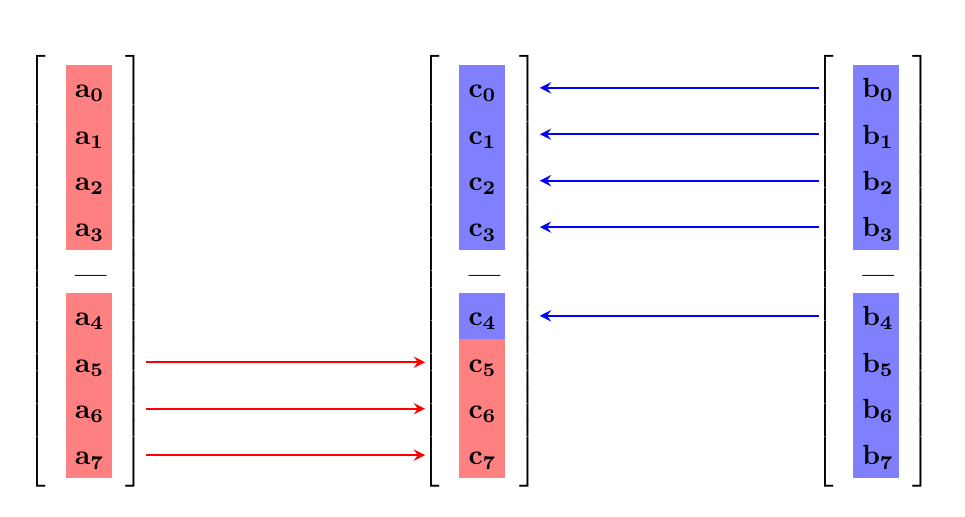
\begin{tikzpicture}[>=stealth,thick,baseline, every node/.style={text height=2ex,text width=1em}]
\plotSwizzleThreeRegisters{blue}{blue}{blue}{blue}{blue}{red}{red}{red}

\draw[->,color=blue]([xshift=-12pt]B-1-1.west)-- ([xshift= 12pt]C-1-1.east);
\draw[->,color=blue]([xshift=-12pt]B-2-1.west)-- ([xshift= 12pt]C-2-1.east);
\draw[->,color=blue]([xshift=-12pt]B-3-1.west)-- ([xshift= 12pt]C-3-1.east);
\draw[->,color=blue]([xshift=-12pt]B-4-1.west)-- ([xshift= 12pt]C-4-1.east);
\draw[->,color=blue]([xshift=-12pt]B-6-1.west)-- ([xshift= 12pt]C-6-1.east);
\draw[->,color=red ]([xshift= 12pt]A-7-1.east)-- ([xshift=-12pt]C-7-1.west);
\draw[->,color=red ]([xshift= 12pt]A-8-1.east)-- ([xshift=-12pt]C-8-1.west);
\draw[->,color=red ]([xshift= 12pt]A-9-1.east)-- ([xshift=-12pt]C-9-1.west);
\end{tikzpicture}




\subsubsection{BlendInRange}

The \cppInline{BlendIndex} function has two template parameters independent of the used register types' size.
Data elements with indices equal or between those 2 values are taken from the second source register. 
All other are taken from the first one.

\subsubsection*{Example:}
\begin{minted}{cpp}
__m256 c = BlendInRange<3, 5>(a, b)
\end{minted}

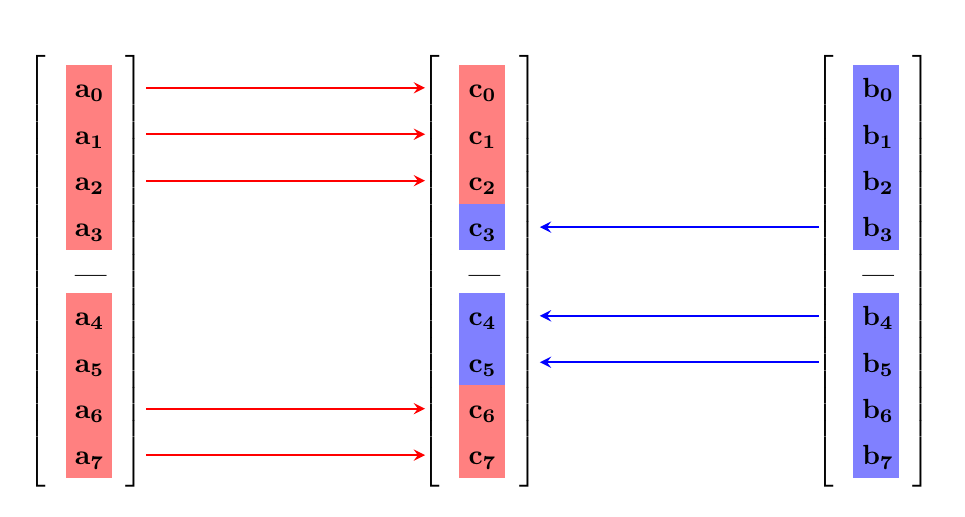
\begin{tikzpicture}[>=stealth,thick,baseline, every node/.style={text height=2ex,text width=1em}]
\plotSwizzleThreeRegisters{red}{red}{red}{blue}{blue}{blue}{red}{red}

\draw[->,color=red ]([xshift= 12pt]A-1-1.east)-- ([xshift=-12pt]C-1-1.west);
\draw[->,color=red ]([xshift= 12pt]A-2-1.east)-- ([xshift=-12pt]C-2-1.west);
\draw[->,color=red ]([xshift= 12pt]A-3-1.east)-- ([xshift=-12pt]C-3-1.west);
\draw[->,color=blue]([xshift=-12pt]B-4-1.west)-- ([xshift= 12pt]C-4-1.east);
\draw[->,color=blue]([xshift=-12pt]B-6-1.west)-- ([xshift= 12pt]C-6-1.east);
\draw[->,color=blue]([xshift=-12pt]B-7-1.west)-- ([xshift= 12pt]C-7-1.east);
\draw[->,color=red ]([xshift= 12pt]A-8-1.east)-- ([xshift=-12pt]C-8-1.west);
\draw[->,color=red ]([xshift= 12pt]A-9-1.east)-- ([xshift=-12pt]C-9-1.west);
\end{tikzpicture}
\subsection{Broadcast functions}

Broadcast operations copy a single value (per lane) from a source register to all data elements (per lane) of the result register.  

\subsubsection{Broadcast}

The \cppInline{Broadcast} function broadcast one value per lane.
The position inside the lane of the data element that should be broadcasted is passed as template parameter.
For multi-lane registers it is also possible to select different positions per lane by providing as many template parameters as the register has lanes.

\vspace{1cm}
\begin{minipage}{\linewidth}
\subsubsection*{Example 1:}
\begin{minted}{cpp}
__m256 b = Broadcast<2>(a)
\end{minted}

\begin{tikzpicture}[>=stealth,thick,baseline, every node/.style={text height=2ex,text width=1em}]
\plotSwizzleTwoRegisters{2}{2}{2}{2}{6}{6}{6}{6}
\draw[->,color=black ]([xshift= 12pt]A-3-1.east)-- ([xshift=-12pt]B-1-1.west);
\draw[->,color=black ]([xshift= 12pt]A-3-1.east)-- ([xshift=-12pt]B-2-1.west);
\draw[->,color=black ]([xshift= 12pt]A-3-1.east)-- ([xshift=-12pt]B-3-1.west);
\draw[->,color=black ]([xshift= 12pt]A-3-1.east)-- ([xshift=-12pt]B-4-1.west);
\draw[->,color=black ]([xshift= 12pt]A-8-1.east)-- ([xshift=-12pt]B-6-1.west);
\draw[->,color=black ]([xshift= 12pt]A-8-1.east)-- ([xshift=-12pt]B-7-1.west);
\draw[->,color=black ]([xshift= 12pt]A-8-1.east)-- ([xshift=-12pt]B-8-1.west);
\draw[->,color=black ]([xshift= 12pt]A-8-1.east)-- ([xshift=-12pt]B-9-1.west);
\end{tikzpicture}
\end{minipage}

\vspace{1cm}
\begin{minipage}{\linewidth}
\subsubsection*{Example 2:}
\begin{minted}{cpp}
__m256 b = Broadcast<0, 3>(a)
\end{minted}

\begin{tikzpicture}[>=stealth,thick,baseline, every node/.style={text height=2ex,text width=1em}]
\plotSwizzleTwoRegisters{0}{0}{0}{0}{7}{7}{7}{7}
\draw[->,color=black ]([xshift= 12pt]A-1-1.east)-- ([xshift=-12pt]B-1-1.west);
\draw[->,color=black ]([xshift= 12pt]A-1-1.east)-- ([xshift=-12pt]B-2-1.west);
\draw[->,color=black ]([xshift= 12pt]A-1-1.east)-- ([xshift=-12pt]B-3-1.west);
\draw[->,color=black ]([xshift= 12pt]A-1-1.east)-- ([xshift=-12pt]B-4-1.west);
\draw[->,color=black ]([xshift= 12pt]A-9-1.east)-- ([xshift=-12pt]B-6-1.west);
\draw[->,color=black ]([xshift= 12pt]A-9-1.east)-- ([xshift=-12pt]B-7-1.west);
\draw[->,color=black ]([xshift= 12pt]A-9-1.east)-- ([xshift=-12pt]B-8-1.west);
\draw[->,color=black ]([xshift= 12pt]A-9-1.east)-- ([xshift=-12pt]B-9-1.west);
\end{tikzpicture}
\end{minipage}


\subsubsection{BroadcastAcrossLanes}

For single lane registers, `BroadcastAcrossLanes` behaves the same as `Broadcast`.
For multi-lane registers, a single value selected by a template parameter is written to all data elements of the result register. 
Keep in mind, that broadcasting across lane boundaries is a rather expensive operation and should only be used if it is really necessary.

\vspace{1cm}
\begin{minipage}{\linewidth}
\subsubsection*{Example:}
\begin{minted}{cpp}
__m256 b = BroadcastAcrossLanes<5>(a)
\end{minted}

\begin{tikzpicture}[>=stealth,thick,baseline, every node/.style={text height=2ex,text width=1em}]
\plotSwizzleTwoRegisters{5}{5}{5}{5}{5}{5}{5}{5}
\draw[->,color=black ]([xshift= 12pt]A-7-1.east)-- ([xshift=-12pt]B-1-1.west);
\draw[->,color=black ]([xshift= 12pt]A-7-1.east)-- ([xshift=-12pt]B-2-1.west);
\draw[->,color=black ]([xshift= 12pt]A-7-1.east)-- ([xshift=-12pt]B-3-1.west);
\draw[->,color=black ]([xshift= 12pt]A-7-1.east)-- ([xshift=-12pt]B-4-1.west);
\draw[->,color=black ]([xshift= 12pt]A-7-1.east)-- ([xshift=-12pt]B-6-1.west);
\draw[->,color=black ]([xshift= 12pt]A-7-1.east)-- ([xshift=-12pt]B-7-1.west);
\draw[->,color=black ]([xshift= 12pt]A-7-1.east)-- ([xshift=-12pt]B-8-1.west);
\draw[->,color=black ]([xshift= 12pt]A-7-1.east)-- ([xshift=-12pt]B-9-1.west);
\end{tikzpicture}
\end{minipage}
\subsection{Exchange}

The \cppInline{Exchange} function modifies the passed registers directly (pass by reference) and does not return a new register.
It exchanges two values between both the registers.
The indices of the corresponding data elements are specified as template parameters.
Note that the cost of this operation is significantly higher if the exchanged values are not in the same register lane. 

\subsubsection*{Example:}
\begin{minted}{cpp}
Exchange<1, 6>(a, b)
\end{minted}

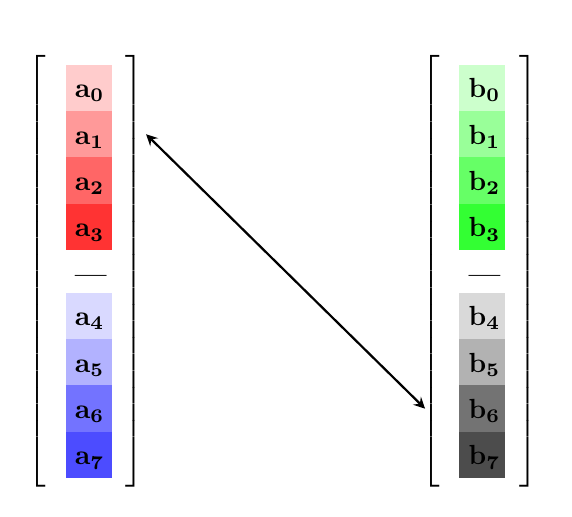
\begin{tikzpicture}[>=stealth,thick,baseline, every node/.style={text height=2ex,text width=1em}]
\matrix [matrix of math nodes,
left delimiter={[},
right delimiter={]},
](A) at (0,0){ 
	|[fill=red!20]|\mathbf{a_{0}}\\
	|[fill=red!40]|\mathbf{a_{1}}\\  
	|[fill=red!60]|\mathbf{a_{2}}\\
	|[fill=red!80]|\mathbf{a_{3}}\\
	\textbf{---}\\
	|[fill=blue!15]|\mathbf{a_{4}}\\
	|[fill=blue!30]|\mathbf{a_{5}}\\
	|[fill=blue!55]|\mathbf{a_{6}}\\
	|[fill=blue!70]|\mathbf{a_{7}}\\
};

\matrix [matrix of math nodes,
left delimiter={[},
right delimiter={]},
](B) at (5,0){ 
	|[fill=green!20]|\mathbf{b_{0}}\\
	|[fill=green!40]|\mathbf{b_{1}}\\  
	|[fill=green!60]|\mathbf{b_{2}}\\
	|[fill=green!80]|\mathbf{b_{3}}\\
	\textbf{---}\\
	|[fill=black!15]|\mathbf{b_{4}}\\
	|[fill=black!30]|\mathbf{b_{5}}\\
	|[fill=black!55]|\mathbf{b_{6}}\\
	|[fill=black!70]|\mathbf{b_{7}}\\
};

\draw[<->,color=black]([xshift= 12pt]A-2-1.east)-- ([xshift=-12pt]B-8-1.west);
\end{tikzpicture}
\hspace{1cm}
result: 
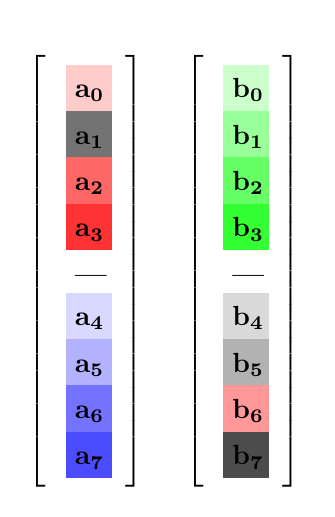
\begin{tikzpicture}[>=stealth,thick,baseline, every node/.style={text height=2ex,text width=1em}]
\matrix [matrix of math nodes,
left delimiter={[},
right delimiter={]},
](A) at (0,0){ 
	|[fill=red!20]|\mathbf{a_{0}}\\
	|[fill=black!55]|\mathbf{a_{1}}\\  
	|[fill=red!60]|\mathbf{a_{2}}\\
	|[fill=red!80]|\mathbf{a_{3}}\\
	\textbf{---}\\
	|[fill=blue!15]|\mathbf{a_{4}}\\
	|[fill=blue!30]|\mathbf{a_{5}}\\
	|[fill=blue!55]|\mathbf{a_{6}}\\
	|[fill=blue!70]|\mathbf{a_{7}}\\
};

\matrix [matrix of math nodes,
left delimiter={[},
right delimiter={]},
](B) at (2,0){ 
	|[fill=green!20]|\mathbf{b_{0}}\\
	|[fill=green!40]|\mathbf{b_{1}}\\  
	|[fill=green!60]|\mathbf{b_{2}}\\
	|[fill=green!80]|\mathbf{b_{3}}\\
	\textbf{---}\\
	|[fill=black!15]|\mathbf{b_{4}}\\
	|[fill=black!30]|\mathbf{b_{5}}\\
	|[fill=red!40]|\mathbf{b_{6}}\\
	|[fill=black!70]|\mathbf{b_{7}}\\
};
\end{tikzpicture}
\subsection{Unpack functions}

The unpack functions copy values from both source registers interleaved into the result register.

\subsubsection{\_mm\_unpacklo}
This function takes from each source register lane the values that belong to the half with the low indices and copies them interleaved into the corresponding lane of the result register.

\subsubsection*{Example:}
\begin{minted}{cpp}
__m256 c = _mm_unpacklo(a, b)
\end{minted}

\begin{tikzpicture}[>=stealth,thick,baseline, every node/.style={text height=2ex,text width=1em}]
\plotSwizzleThreeRegisters{\colorA{0}}{\colorB{0}}{\colorA{1}}{\colorB{1}}{\colorA{4}}{\colorB{4}}{\colorA{5}}{\colorB{5}}

\draw[->,color=black ]([xshift= 12pt]A-1-1.east)-- ([xshift=-12pt]C-1-1.west);
\draw[->,color=black ]([xshift= 12pt]A-2-1.east)-- ([xshift=-12pt]C-3-1.west);
\draw[->,color=black ]([xshift=-12pt]B-1-1.west)-- ([xshift=12pt]C-2-1.east);
\draw[->,color=black]([xshift=-12pt]B-2-1.west)-- ([xshift= 12pt]C-4-1.east);
\draw[->,color=black ]([xshift= 12pt]A-6-1.east)-- ([xshift=-12pt]C-6-1.west);
\draw[->,color=black ]([xshift= 12pt]A-7-1.east)-- ([xshift=-12pt]C-8-1.west);
\draw[->,color=black ]([xshift=-12pt]B-6-1.west)-- ([xshift=12pt]C-7-1.east);
\draw[->,color=black]([xshift=-12pt]B-7-1.west)-- ([xshift= 12pt]C-9-1.east);
\end{tikzpicture}


\subsubsection{\_mm\_unpackhi}
This function takes from each source register lane the values that belong to the half with the high indices and copies them interleaved into the corresponding lane of the result register.

\subsubsection*{Example:}
\begin{minted}{cpp}
__m256 c = _mm_unpackhi(a, b)
\end{minted}

\begin{tikzpicture}[>=stealth,thick,baseline, every node/.style={text height=2ex,text width=1em}]
\plotSwizzleThreeRegisters{\colorA{2}}{\colorB{2}}{\colorA{3}}{\colorB{3}}{\colorA{6}}{\colorB{6}}{\colorA{7}}{\colorB{7}}

\draw[->,color=black ]([xshift= 12pt]A-3-1.east)-- ([xshift=-12pt]C-1-1.west);
\draw[->,color=black ]([xshift= 12pt]A-4-1.east)-- ([xshift=-12pt]C-3-1.west);
\draw[->,color=black ]([xshift=-12pt]B-3-1.west)-- ([xshift=12pt]C-2-1.east);
\draw[->,color=black]([xshift=-12pt]B-4-1.west)-- ([xshift= 12pt]C-4-1.east);
\draw[->,color=black ]([xshift= 12pt]A-8-1.east)-- ([xshift=-12pt]C-6-1.west);
\draw[->,color=black ]([xshift= 12pt]A-9-1.east)-- ([xshift=-12pt]C-8-1.west);
\draw[->,color=black ]([xshift=-12pt]B-8-1.west)-- ([xshift=12pt]C-7-1.east);
\draw[->,color=black]([xshift=-12pt]B-9-1.west)-- ([xshift= 12pt]C-9-1.east);
\end{tikzpicture}





\subsection{Permute}
\subsection{Shuffle}
\subsection{Insert}
\subsection{Lane Permutations}

\section{Transpose functions}


\end{document}